\chapter{Data Structures for Hierarchical Phrase-Based Translation Grammars}
\chaptermark{Data Structures for Hiero Grammars}
\label{chap:hfile}

% TODOFINAL grep map, reduce and italicize
% TODOFINAL bottom margin too big, make it smaller
% TODOFINAL for viva: reread hbase book doc on hfile
% TODOFINAL grep for model (in this chapter) and clarify if needed
% TODOFINAL grep for backoff back-off
% TODOFINAL grep for gram. use $n$-gram consistently
% TODOFINAL grep for filter filtering usage
% TODOFINAL grep for future and add it to future work in conclusion
% TODOFINAL check with Bill the 2000 words per minute ??????
% TODOFINAL check abbreviation space after dot (i.e. e.g. etc.)
% TODOFINAL grep for corpus (parallel corpus) and replace with parallel text
% TODOFINAL grep for MapReduce feature
% TODOFINAL grep for collection specific and add hyphen
% TODOFINAL (done ?) subsubsections to be numbered
% TODOFINAL grep for word alignment and add or not hyphen
% TODOFINAL grep for Hfile wrongly capitalized
% TODOFINAL try to remove all mentions of hbase
% TODOFINAL check for duplicates in bibliography
% TODOSUBMIT introduce MapReduce in background chapter
% TODOFINAL check title casing
% TODOFINAL check usage of word ``model''
% TODOFINAL check usage of past tense and present tense

We have seen in \autoref{chap:smt} that the main components of an SMT
system are the translation model and the language model. The translation
model is trained on parallel text while the language model is typically
trained on the target side of the parallel text and possibly additional
monolingual target text. It has been shown that increasing the amount
of parallel
text~\citep{pino-iglesias-degispert-blackwood-brunning-byrne:2010:WMT}
and increasing the amount of monolingual
text~\citep{brants-popat-xu-och-dean:2007:EMNLP-CoNLL}
is beneficial for translation quality.

Monolingual and parallel text availability and distributed computing techniques
have allowed SMT
researchers to build ever larger language models and
translation models, based on very large amounts of data.
However, decoders need to be
able to retrieve information, such as $n$-gram conditional
probabilities or translation grammar rules, efficiently from these models to be able to
translate an input sentence or a set of input sentences in a reasonable amount
of time. For online systems such as the commercial systems
mentioned in \autoref{chap:intro}, translation even needs to be carried out in % TODOFINAL for online systems: maybe refer to intro (Google Translate, etc.)
\emph{real time}, i.e.\ for example with a speed of 2000 words translated per minute.

Therefore SMT models need to be stored in a data structure
that supports efficient querying and is scalable. We introduce a solution
that addresses these two requirements and that has the advantage that
it reuses an existing framework in order to ease the implementation.
We store translation models as a set of key-value pairs in an
HFile\footnote{\url{http://hbase.apache.org}}. We apply this
strategy in order to retrieve relevant rules
from a hierarchical phrase-based grammar at the test set level. We compare our
approach to alternative strategies and show that our approach
offers competitive performance in terms
of speed, memory and simplicity~\citep{pino-waite-byrne:2012:PBML}. We
have made software written
for this work
available online.\footnote{\url{https://github.com/jmp84/ruleXtract} (branch PBML-2012)}

\section{Introduction}
\label{sec:hfileIntro}

Current machine translation research is characterised by increasing amounts
of available data. For example, \autoref{fig:wmtdata} shows that
for the WMT machine translation
workshop~\citep{bojar-buck-callisonburch-federmann-haddow-koehn-monz-post-soricut-specia:2013:WMT}
French-English constrained track translation shared task, the English side of parallel
data has increased from 13.8M tokens in 2006 to 1012.7M tokens in 2013, and that
available English monolingual data has increased from 27.5M tokens to 6852.7M
tokens over the same period.
%
\begin{figure}
  \begin{center}
    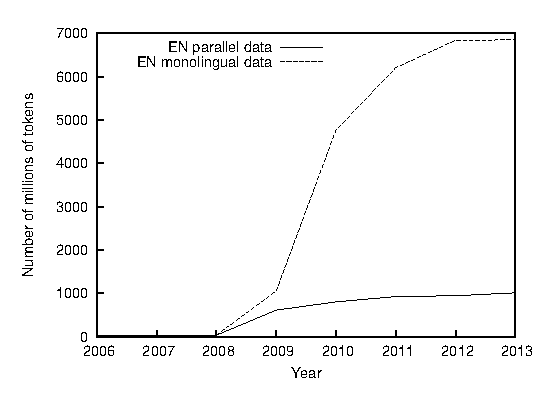
\includegraphics{figures/wmt/wmtdata.eps}
    \caption{Number of English tokens (in millions) in parallel and monolingual
      data available for the WMT French-English constrained track translation
      shared task for the years 2006 to 2013.}
    \label{fig:wmtdata}
  \end{center}
\end{figure}
%
Along with growing amounts of data, the use of more powerful computers
and distributed computing models such as
% rather than to paper
MapReduce~\citep{dean-ghemawat:2008:ACM,lin-dyer:2010:book} has enabled machine % TODOSUBMIT refer to background
translation researchers to build larger statistical machine translation models.
%Indeed, MapReduce was originally designed to process large datasets for parallelizable
%algorithms.
%
% notes on brants et al 2007 paper
% uses cutoffs
% p(w_i | w_{i - k + 1}^{i - 1}) = rho(w_{i - k + 1}^i) if w_{i - k + 1}^i is found
% = lambda(w_{i - k + 1}^{i - 1}) p(w_{i - k + 2}^i) o/w
% sb not a probability not a problem: it's just a feature scaled appropriately by mert
% vocabulary generation
% word to integer id conversion
% cutoff: words occurring less than threshold mapped to UNK
% vocabulary generation done with mapreduce
% mapreduce program is simply the canonical word count program
% generation of n-grams
% same as word count but with ngrams
% partition function that computes hash on first words of the n-gram
% use hash based on first 2 words
% needs to store unigram counts on all shards, as well as the corpus size N
% language model generation
% this is done online from what i understand
% given an n-gram, a particular shard is contacted
% there is further sharding from ngrams and their count
% but the last two words of the n-grams and also unigrams need to be stored again
% decoder architecture: store 1000-10000 ngrams then send them
% to the servers and compute sb probas on the fly
% search procedure
% current graph. then advance one word in source language,
% expand active hypotheses, queue up necessary ngrams,
% ask for scores, score expanded hypotheses and prune
%
MapReduce has thus been applied to various steps of the
translation
pipeline:
word alignment~\citep{dyer-cordova-mont-lin:2008:WMT},
translation model building~\citep{dyer-cordova-mont-lin:2008:WMT}
and
language
modelling~\citep{brants-popat-xu-och-dean:2007:EMNLP-CoNLL}.
We review these applications of MapReduce in more detail
in \autoref{sec:relatedwork}. The challenge is to find
effective modelling techniques that can be implemented
in the MapReduce framework.

However, once SMT models such as language models and translation
grammars are built, either with MapReduce
or some other method, the models must be made usable
by translation decoders, which only need a fraction of the information
contained in those models to be able to translate an input source sentence or a
set of input source sentences. For example, in translation from French to
English with a phrase-based
model (see \autoref{sec:phraseBasedTranslation}),
given an input sentence \emph{Salut toi}, we only need to know the
translation probabilities the translation model assigns to translations of
the words
\emph{Salut} and \emph{toi} and to translations of the phrase \emph{Salut toi}.
Similarly, given a test set, a decoder
only needs to retrieve the rules whose source side matches part of one of the source
sentences in the test set to be able to generate hypotheses.
With large models, simply retrieving relevant rules together with their
translation
probabilities becomes a challenge.

In the system
described by \citet{iglesias-degispert-banga-byrne:2009:NAACL},
given a training parallel corpus, rules are extracted and target
phrases and hierarchical phrases with counts are stored on disk.
Then, given an input test set, rules are extracted from the parallel
corpus a second time. Only rules relevant to the test set
are retained: source sides of phrase-based rules have to match
an $n$-gram from the test set and consecutive terminals
in source sides of hierarchical rules also have to match
an $n$-gram from the test set. As a consequence, some hierarchical
rules are never used in decoding. % TODOFINAL give an example
Source sides and rules together with their counts are kept
in memory using hash map datastructures, target sides with counts
are loaded from disk as precomputed in the first step, so that
source-to-target and target-to-source probabilities can be computed.

This
method becomes progressively slower with larger amounts of data
because it requires extracting rules from the training parallel corpus
and recomputing translation probabilities
each time we translate a new test set or a new
sentence. We
would like to improve on this design for more rapid experimentation. We also would like
to use a computing infrastructure that requires minimal maintenance. For example,
HBase\footnote{\url{http://hbase.apache.org}}, the open source non-relational database
implementation of
BigTable~\citep{chang-dean-ghemawat-hsieh-wallach-burrows-chandra-fikes-gruber:2008:ACM}, has been applied to the use of distributed language
models~\citep{yu:2008:mastersthesis}. However, we wish to address the question
whether we can adapt this infrastructure to our purposes with minimal
effort and without having to resort to database maintenance.
Rule filtering, i.e. the retrieval of rules relevant to the translation
of a test set or a sentence, is an essential step in our pipeline that can be a
bottleneck. Our goal is to reduce its processing time from several hours to a
few minutes.

In this chapter, we address the problem of retrieving relevant rules with their
translation probabilities. We report on investigations into
storing the model in the HFile data
structure. To our knowledge, this is the first
detailed proposed implementation of translation model storage and
filtering using HFile data structures. We find that this approach
offers a good compromise
between speed, performance and ease of implementation. The infrastructure necessary
for filtering is lightweight and requires the use of only one machine. We will
apply this approach to test set rule filtering prior
to decoding. We will discuss alternative
strategies as well as their strengths and weaknesses in terms of speed and
memory usage. In \autoref{sec:relatedwork}, we will review approaches that
have been used for model building and model filtering.
The HFile data structure that is used to
store models will be presented in \autoref{sec:hfile}.
In \autoref{sec:rulextractMapReduce}, we detail our custom implementation
of rule extraction and translation model estimation using
MapReduce. Our method and
alternative strategies for rule filtering are compared empirically in
\autoref{sec:rulextract}. We conclude in \autoref{sec:conclusion}.

\section{Related Work}
\label{sec:relatedwork}

In this section, we review applications of MapReduce to
the translation pipeline as well as techniques for storing
and retrieving from SMT models.

\subsection{Applications of MapReduce to SMT}
\label{sec:applicationsMapReduceSMT}

\citet{brants-popat-xu-och-dean:2007:EMNLP-CoNLL}
introduce a new smoothing method called
\emph{Stupid Backoff} (see \autoref{sec:stupidBackoffSmoothing}).
The Stupid Backoff smoothing scheme is recalled in \autoref{eq:stupidBackoffSchemeReminder}:
%
\begin{equation}
  p_{\text{stupid backoff}}(w_i \mid w_{i - n + 1}^{i - 1}) =
  \begin{cases}
    \frac{c(w_{i - n + 1}^i)}{c(w_{i - n + 1}^{i - 1})} & \text{if } c(w_{i - n + 1}^i) > 0 \\
    \alpha \, p_{\text{stupid backoff}}(w_i \mid w_{i - n + 2}^{i - 1}) & \text{if } c(w_{i - n + 1}^i) = 0
  \end{cases}
  \label{eq:stupidBackoffSchemeReminder}
\end{equation}
%
With respect to the traditional backoff scheme, the Stupid Backoff
scheme uses no discounting and simply uses relative frequency
for the non backed-off score and the backed-off score
scaling parameter is independent of
the $n$-gram history.
Therefore this scheme does not define a conditional probability
distribution % TODOFINAL add the word conditional in background
over a word given its history.

The Stupid Backoff language model building and application fit the
MapReduce framework well. The input to language model building
is a large monolingual corpus. The first step is to build
a vocabulary. This is done with the canonical example of word
counting with MapReduce. Counts % (see TODOSUBMIT refer to background)
are needed in order to remove words occurring less than a threshold
from the vocabulary. The second step is to obtain $n$-grams and their
count. This is done again with MapReduce, and the \emph{map} and \emph{reduce}
functions are analogous to the ones defined for word counting but this time
unigrams are replaced by $n$-grams.
For $n$-gram counting, the partition, or sharding, function hashes
on the first two words of each $n$-gram. In addition, unigram counts
and the total size of the corpus is available in each partition, i.e.
to each reducer. This allows relative frequencies to be computed.
\citet{brants-popat-xu-och-dean:2007:EMNLP-CoNLL} also
demonstrate
that for large amounts of monolingual data, i.e. above 10 billion
tokens, Stupid Backoff smoothing and Kneser-Ney smoothing perform comparably.
In addition, only
Stupid Backoff smoothing can be scaled to datasets
with more than 31 billion tokens. The scalability of Kneser-Ney
smoothing has been improved in recent work~\citep{heafield-pouzyrevsky-clark-koehn:2013:ACL}.\footnote{see also \url{http://kheafield.com/code/kenlm/estimation/}, Scalability section}

\citet{dyer-cordova-mont-lin:2008:WMT}
observe that translation model estimation has become prohibitive
on a single core and that existing \emph{ad hoc} parallelization
algorithms may be more fragile than using an existing framework such
as the Hadoop implementation of
MapReduce.\footnote{\url{https://hadoop.apache.org/}}
They provide solutions to word alignment model
estimation and translation rule extraction and estimation using MapReduce
and demonstrate the scalability of their method.

The convenience
of the MapReduce framework for parallelization has led to the building
of end-to-end toolkits for entire phrase-based~\citep{gao-vogel:2010:PBML} and
hierarchical phrase-based models~\citep{venugopal-zollmann:2009:PBML}
for translation using the MapReduce framework.

\subsection{SMT Models Storage and Retrieval Solutions}

We now review techniques appearing in the literature that have been used to
store SMT models and to retrieve the information needed in translation from
these models. SMT models are usually discrete probabilistic models and can
therefore be represented as a set of key-value pairs. To obtain relevant
information from a model stored in a certain data structure, a set of keys called a
\emph{query set} is formed; each key in this query set is then sought in that
datastructure. Strategies include:
%
\begin{itemize}
  \item storing the model as a simple data structure in memory
  \item storing the model in a text file
  \item storing the model in more complicated data structures such as
    tries~\citep{fredkin:1960:ACM} (in memory or disk)
  \item storing fractions of the entire model
  \item storing data as opposed to a precomputed model
  \item storing models in a distributed fashion
\end{itemize}
%
Each of these
strategies is discussed below.

In some cases, it may be possible to fit a model into RAM. In
this case the model can be stored as a memory associative array, such as a hash
table. In-memory storage allows allows for faster query retrieval than
on-disk storage, however only smaller models will fit in memory.
In-memory storage has been used to store model
parameters between iterations of expectation-maximisation for word
alignment~\citep{dyer-cordova-mont-lin:2008:WMT,lin-dyer:2010:book}.
% TODOFINAL somehow cite work by matei zaharia

For larger models, the set of key-value pairs can be stored as a table in a
single text file on local disk. Values for keys in the query set can be retrieved
by scanning through the entire file. For each key in the file, its membership is
tested in the query set. This is the approach adopted in the \emph{Joshua 5.0}
decoder~\citep{post-ganitkevitch-orland-weese-cao-callisonburch:2013:WMT}\footnote{Inferred from the decoder training
scripts available at \url{http://joshua-decoder.org/5.0/index.html}.}, which
uses regular expressions or $n$-grams to test
membership (see \autoref{sec:joshuaFiltering}).
\citet{venugopal-zollmann:2009:PBML} use MapReduce to scan a file concurrently:
the \emph{map} function tests if the vocabulary of a rule matches the
vocabulary of a test set.

The model can also be stored using a trie associative
array~\citep{fredkin:1960:ACM}. A trie is a type of tree where each node
represents a shared prefix of a set of keys represented by the child nodes. Each
node only stores the prefix it represents. The keys are therefore compactly
encoded in the structure of the trie itself. Querying the trie is a
$\mathcal{O}(\log(n))$ operation, where $n$ is the number of keys in the
dataset. The trie may also be small enough to fit in physical memory to further
reduce querying time. \citet{zens-ney:2007:HLTNAACL} use tries
to store a phrase-based grammmar. All the source phrases are represented
in a trie stored on disk. Only relevant parts of the trie are loaded into
memory when a source phrase is sought.
\citet{ganitkevitch-cao-weese-post-callisonburch:2012:WMT} extend this
approach to store hierarchical phrase-based grammars. Both
source sides and target sides are stored in a packed representation of a trie.
Packed tries have also been applied for storing language
models~\citep{pauls-klein:2011:HLTACL,heafield:2011:WMT}.

It is also possible to create a much smaller approximate version of the model.
\citet{talbot-osborne:2007:ACL} represent a set of $n$-grams as a Bloom
filter~\citep{bloom:1970:ACM}.
They first use a standard Bloom filter to define a binary feature that
indicates whether an $n$-gram was seen in a monolingual corpus. They
also use a Bloom filter to encode $n$-grams together with quantized counts
in order to define a multinomial feature, that is a feature
with a finite set of possible values---in this case the quantized values. Both these data structure can
substantially reduce the disk space and memory usage with respect to lossless
representations of language models. However, they allow
false positives for $n$-gram
membership queries and overestimates of $n$-gram quantized counts. The authors
demonstrate that the features they introduce are useful in translation, despite
this lack of exactness.
In a related publication~\citep{talbot-osborne:2007:EMNLP-CoNLL}, the authors
demonstrate how these techniques can be used as a replacement to represent
a smoothed language model. \citet{talbot-brants:2008:ACL} use a Bloomier
filter~\citep{chazelle-kilian-rubinfeld-tal:2004:ACM-SIAM}
to represent $n$-grams and necessary statistics such as probabilities and backoff
weights. Unlike Bloom filters that only support Boolean characteristic
functions on a set, Bloomier filters support arbitrary functions, in this case
a mapping between an $n$-gram and its statistics. False positives can still occur
but for true positives, correct statistics are retrieved.

% TODOFINAL explain this better
%talbot-brants acl
%represent ngrams, proba, backoff with hash
%randomized language model
%kind of error: false positive but when ngram found, params are correct
%based on bloomier filter
%bloomier filter allows for arbitrary function as opposed to binary function

\citet{guthrie-hepple:2010:EMNLP} propose an extension to previous work
on randomized language models~\citep{talbot-osborne:2007:EMNLP-CoNLL} which prevents
the random corruption of model parameters but does not stop the random
assignment of parameters to unseen $n$-grams.
\citet{levenberg-osborne:2009:EMNLP} extend randomised language models to
stream-based language models. Another way of building a smaller approximate
version of a model is to retain items with high frequency counts from a stream
of data~\citep{manku-motwani:2002:VLDB}. This technique has been applied to
language modelling~\citep{goyal-daumeiii-venkatasubramanian:2009:NAACL} and
translation rule extraction~\citep{przywara-bojar:2011:PBML}. 


%talbot acl
%use bloom filter
%use standard bloom filter to test whether ngram was seen
%use log-frequency bloom filter to add frequency information
%ngram counts are quantised
%log frequency bloom filter: (ngram,1) (ngram,2) ... (ngram, quantizedcount(ngram)) inserted into the BF
%at retrieval time, we get back a count equal or greater than the actual quantized count
%trick to reduce error: c(w1-wn) < min(c(w1-wn-1), c(w2,wn))
%bloom filter language model test: use binary feature
%log-frequency bf lm: use the quantized count
%experiments: those features are useful in translation

%talbot emnlp
%this time not just binary features, but the whole lm estimated
%still use a log-frequency bf
%new: expected value of count
%E[c(x)|qc(x)=j] = (b^{j-1} + b^j - 1) / 2
%ccl: replacement for usual lm, use less space and memory

Instead of doing some precomputation on a dataset, it is possible to compute
the sufficient
statistics at query time using a suffix array~\citep{manber-myers:1990:SIAM}, so
that the model can be estimated only when needed. A suffix array is a sequence of
pointers to each suffix in a training corpus. The sequence is sorted with
respect to the lexicographic order of the referenced suffixes. Suffix arrays
have been used for computing statistics for language
models~\citep{zhang-vogel:2006:techreport}, phrase-based
systems~\citep{callisonburch-bannard-schroeder:2005:ACL,zhang-vogel:2005:EAMT},
and hierarchical phrase-based systems~\citep{lopez:2007:EMNLP-CoNLL}.
\citet{callisonburch-bannard-schroeder:2005:ACL} store both the source side
and the target side of a parallel corpus in two suffix arrays. They also maintain
an index between a position in the source or target side of the corpus and the
sentence number. During decoding, all occurrences of a source phrase
are located in the suffix array representing the source side of the corpus.
This produces a source marginal count. For each of these occurrences, the corresponding
sentence pair and word alignment are retrieved and rules are extracted. This produces
a rule count, which is normalized with the source marginal count to produce a
source-to-target probability. \citet{lopez:2007:EMNLP-CoNLL} extends this approach
to address the grammar extraction and estimation of hierarchical rules.
Note that the use of suffix arrays for translation model estimation only
supports the computation of source-to-target probabilities.

% TODOFINAL explain suffix array better
%suffixarray callisonburch
%suffix array for source corpus
%suffix array for target corpus
%index between sentence number and position in corpus (src and target)
%word alignment

%compute s2t probability
%locate all occurrences of f: gives c(f)
%for each occurrence of f, retrieve sentence pair and alignment
%run extraction: gives c(f, e)
%compute c(f, e) / c(f)

Finally, some approaches store language models in a distributed fashion.
We saw in \autoref{sec:applicationsMapReduceSMT} how a Stupid Backoff language
model can be built. After relative frequencies have been computed, another
partition function that hashes on the last two words of an $n$-gram is applied
so that backoff operations can be done withing the same partition.
At decoding time, the decoder architecture is modified in order
to request a batch of $n$-grams rather than a single $n$-gram.
The stupid backoff language model building can be scaled
to a corpus of 2 trillion tokens and the language model distributed
application can be made real time.

\citet{zhang-hildebrand-vogel:2006:EMNLP} propose a distributed large language
model backed by suffix arrays. HBase has also been used to build a distributed
language infrastructure~\citep{yu:2008:mastersthesis}. The method we propose to
use is closely related to the latter but we use a more lightweight
infrastructure than HBase. In addition, it is also possible to apply our method
to language model querying~\citep{pino-waite-byrne:2012:PBML}, which
demonstrates the flexibility of the infrastructure.

\section{HFile Description}
\label{sec:hfile}

We now describe the data structure we use to store models and we review relevant
features to the design of our system. To store a model represented as key-value
pairs, we use the HFile file format,\footnote{\url{http://hbase.apache.org}} which is
a open source reimplementation of the SSTable file
format~\citep{chang-dean-ghemawat-hsieh-wallach-burrows-chandra-fikes-gruber:2008:ACM}.
The HFile format is a lookup table with key and value columns. The entries are free
to be an arbitrary string of bytes of any length. The table is sorted
lexicographically by the key byte string for efficient record retrieval by key.

\subsection{HFile Internal Structure}

% TODOFINAL read SSTable description
% TODOFINAL check whether blocks are plural or singular

\paragraph{High Level Structure} As can be seen in \autoref{fig:hfile},
the HFile internal structure is divided into blocks. There are various types of
block, depending on the kind of information a block contains.
In order to
distinguish block types, the first 8 bytes of a
block will indicate its type. The blocks are grouped into
three parts. The first part (top) is organised into
data blocks interleaved with leaf data index blocks and Bloom blocks.
The second part (middle) consists of intermediate data index blocks.
The third part (bottom) consists of metadata: root data index blocks, a file
information block and a Bloom filter index block.

\paragraph{Index Blocks} The root data index blocks map keys to their
relevant intermediate data index block, indicated by
an offset. In turn, an intermediate data index block
maps keys to their relevant leaf data index block, again indicated by an offset.
Finally, a leaf data index block maps keys to their relevant data block,
still indicated by an offset. The same mechanism is employed for the Bloom filter.
The Bloom filter index block maps keys to their relevant Bloom block.

\paragraph{Block Size Configuration} The block size is
configurable, with a default size of 64KB. Note that HFile blocks are not to be
confused with Hadoop Distributed File System (HDFS) blocks whose default size is
64MB.

\paragraph{Block Compression} The HFile format allows for
the blocks to be compressed. The choice of compression codec is selected when
the file is created. We choose the GZip compression
codec~\citep{Deutsch:1996:ZCD:RFC1950} for all our % TODOFINAL check that the gzip cite is correct
experiments.
%Block compression is also used in other related
%software~\citep{pauls-klein:2011:HLTACL}. % TODOFINAL reread paper and elaborate

\begin{figure}
  \begin{center}
    \begin{tabular}{|l|}
      \hline
      \rowcolor[gray]{0.85}
      Data Block \\
      \hline
      \rowcolor[gray]{0.85}
      ... \\
      \hline
      \rowcolor[gray]{0.95}
      Leaf Data Index Block / Bloom Block \\
      \hline
      \rowcolor[gray]{0.85}
      ... \\
      \hline
      \rowcolor[gray]{0.85}
      Data Block \\
      \hline
      \rowcolor[gray]{0.85}
      ... \\
      \hline
      \rowcolor[gray]{0.95}
      Leaf Data Index Block / Bloom Block \\
      \hline
      \rowcolor[gray]{0.85}
      ... \\
      \hline
      \rowcolor[gray]{0.85}
      Data Block \\
      \hline
      \hline
      \rowcolor[gray]{0.9}
      Intermediate Data Index Blocks \\
      \hline
      \hline
      \rowcolor[gray]{0.7}
      Root Data Index Blocks \\
      \hline
      \rowcolor[gray]{0.7}
      File Info Block \\
      \hline
      \rowcolor[gray]{0.7}
      Bloom Filter Index Block \\
      \hline
    \end{tabular}
    \caption[Caption for LOF]{HFile internal structure.\footnotemark \ The
      structure is divided into three parts. In the first part, data blocks
      are interspersed with leaf data index blocks and Bloom blocks. The second
      part contains intermediate data index blocks. The third part consists
      of metadata: root data index blocks, file format information and a Bloom
      filter index block.}
    \label{fig:hfile}
  \end{center}
\end{figure}

\footnotetext{After \url{http://hbase.apache.org/book/book.html} (simplified)}

\subsection{Record Retrieval}
\label{sec:recordRetrieval}

When the HFile is opened for reading, the root data index blocks are loaded into memory.
To retrieve a value from the HFile given a key, the appropriate intermediate
index block is located by a binary search through the root data index. Binary
searches are conducted on the intermediate and leaf index blocks to identify the
data block that contains the key. The identified data block is then loaded off the disk
into memory and the key-value record is retrieved by scanning the data block
sequentially.

\subsection{Bloom Filter Optimization for Query Retrieval}
\label{sec:bloomFilterOptimization}

It is possible to query for a key that is not contained in the HFile. This very
frequently happens in translation because of language data sparsity: in our case,
because keys are $n$-grams of terminals and nonterminals, the number of possible
keys is exponential in the size of the vocabulary, and many of these
will not have been observed in any rule extracted from training data.

Querying
the existence of a key is expensive as it involves all the operations
described in \autoref{sec:recordRetrieval}: loading and binary
searching the root data index,
loading and binary searching an intermediate data index block,
loading and binary searching
a leaf data index block and finally loading and scanning a data block.

For fast existence check queries, the HFile format allows
the inclusion of an optional Bloom filter~\citep{bloom:1970:ACM}. A Bloom filter
provides a probabilistic, memory efficient representation of the key set with a
$\mathcal{O}(1)$ membership test operation. The Bloom filter may provide a false
positive, % TODOFINAL expand on Bloom filters somewhere either background or here
but never a false negative, for existence of a key in the HFile.
Therefore, it is safe to use in our setting as some keys will be looked
up in the HFile even though they are not present, but the situation
where keys that are in the HFile are not looked up will not happen.

For a large
HFile, the Bloom filter may also be very large. Therefore the  Bloom filter is
also organised into blocks called Bloom blocks. Each block contains a smaller
Bloom filter that covers a range of keys in the HFile. Similar to the root data
index, a Bloom index is constructed. To check for the
existence of a key, a binary search is conducted on the Bloom index, the
relevant Bloom block is loaded, and the membership test performed.

Unlike work on Bloom filter language
model~\citep{talbot-osborne:2007:ACL,talbot-osborne:2007:EMNLP-CoNLL}, this
filter only tests the existence of a key and does not return any statistics from
the value. If a membership test is positive, a usual key search will
still be carried out. During the execution of a query, two keys may
reference the same index or Bloom blocks. To prevent these blocks from being
repeatedly loaded from disk, the blocks are cached after reading.

\subsection{Local Disk Optimization}

The HFile format is designed to be used with HDFS, a distributed file system
based on the Google File System~\citep{ghemawat-gobioff-leung:2003:OSP}. Large
files are split into HDFS blocks that are stored on many nodes in a cluster.
However, the HFile format can also be used completely independently of HDFS. If
its size is smaller than local disk space, the entire HFile can be stored on the local
disk of one machine and accessed through the machine's local file system. We
report in \autoref{sec:rulextract} that using local disk
is faster than using HDFS.

\subsection{Query sorting optimization}
\label{sec:querySortingOptimization}

Prior to HFile lookup, we sort keys in the query set lexicographically. If two
keys in the set of queries are contained in the same block, then the block is
only loaded once. In addition, the computer hardware and operating system allow
further automatic improvements to the query execution. Examples of these
automatic improvements include reduced disk seek time,
caching data from
disk by the operating system,\footnote{The Linux Documentation Project, The File System, \url{http://tldp.org}}
or CPU caching data from main memory~\citep{patterson-hennessy:2005:COA}.

\section{Hierarchical Rule Extraction with MapReduce}
\label{sec:rulextractMapReduce}

In the previous section, we have described the HFile format. We will use
this format to store a translation grammar. In this
section, we describe how we generate this grammar and produce the HFile
that represents the grammar.
We describe a MapReduce implementation of hierarchical grammar
extraction and estimation. The implementation is an
extension of \emph{Method 3} described by
\citet{dyer-cordova-mont-lin:2008:WMT}, which was originally developped
to estimate translation probabilities for phrase-based models.
Using the MapReduce notation introduced
in \autoref{sec:mapReduceInSMT} (TODOSUBMIT: still missing mapreduce background section),
we can describe the grammar extraction and estimation
as a series of MapReduce jobs, summarized in
\autoref{fig:ruleXtractionPipeline}.
%
\begin{figure}
  \tikzstyle{MapReduceJob} = [rectangle, draw, fill=blue!20, rounded corners,
    align = left, text width = 3.5cm]
  \tikzstyle{JobInputOutput} = [draw, ellipse,fill=red!20,
    align = left, text width = 2.9cm]
  \tikzstyle{line} = [draw, very thick, color=black!50, -latex']

%\begin{center}
\begin{tikzpicture}[node distance = 2.2cm]
  \begin{normalsize}
    % Place nodes
    \node [JobInputOutput, text width = 6cm] (corpus) {
      $k_1$ : metadata \\
      $k_2$ : word-aligned sentence pair
    };
    \node [MapReduceJob, below of=corpus, text width = 7cm] (extract) {
      \textbf{Rule Extraction} (see \autoref{sec:hierruleextract}) \\
      \emph{map} : extract rules \\
      \emph{reduce} : none};
    \node [JobInputOutput, below of=extract] (rules) {
      $k_1$ : rule \\
      $k_2$ : metadata};
    \node [MapReduceJob, below left = 1cm and -1.5cm of rules, text width = 6.5cm] (s2t) {
      \textbf{Source-to-target Probability} \\
      \emph{map} : output (\emph{src}, (\emph{trg}, 1)) \\
      \emph{reduce} : sum \emph{trg} counts, normalize};
    \node [MapReduceJob, below right = 1cm and -1.5cm of rules, text width = 6.5cm] (t2s) {
      \textbf{Target-to-source Probability} \\
      \emph{map} : output (\emph{trg}, (\emph{src}, 1)) \\
      \emph{reduce} : sum \emph{src} counts, normalize};
%    \node [MapReduceJob, below = 1.2cm of rules] (other) {\textbf{Other MapReduce Feature}};
    \node [JobInputOutput, below = 0.7cm of s2t, text width = 4.4cm] (rulesPlusS2t) {
      $k_1$ : rule \\
      $k_2$ : source-to-target pr};
    \node [JobInputOutput, below = 0.7cm of t2s, text width = 4.4cm] (rulesPlusT2s) {
      $k_1$ : rule \\
      $k_2$ : target-to-source pr};
%    \node [JobInputOutput, below = 1.7cm of other] (rulesPlusOther) {$k_1$: rule \\
%                                                                   $k_2$: other feature};
    \node [MapReduceJob, below = 5.7cm of rules, text width = 8.5cm] (merge) {
      \textbf{Merge} \\
      \emph{map} : output (\emph{src}, (\emph{trg}, feature)) \\
      \emph{reduce} : output (\emph{src}, list of \emph{trg} and features)};
    \node [JobInputOutput, below = 1cm of merge, text width = 5cm] (ruleAllFeatures) {
      $k_1$ : \emph{src} \\
      $k_2$ : list of \emph{trg} and features};
    % Draw edges
    \path [line] (corpus) -- (extract);
    \path [line] (extract) -- (rules);
    \path [line] (rules) -- (s2t);
    \path [line] (rules) -- (t2s);
%    \path [line] (rules) -- (other);
    \path [line] (s2t) -- (rulesPlusS2t);
    \path [line] (t2s) -- (rulesPlusT2s);
%    \path [line] (other) -- (rulesPlusOther);
%    \path [line] (rulesPlusOther) -- (merge);
    \path [line] (rulesPlusS2t) -- (merge);
    \path [line] (rulesPlusT2s) -- (merge);
    \path [line] (merge) -- (ruleAllFeatures);
    \end{normalsize}
\end{tikzpicture}
%\end{center}
\caption{Translation grammar extraction and estimation pipeline as a series of MapReduce jobs. Ellipses
represent (intermediate) input/output of MapReduce jobs. Rectangles represent
MapReduce jobs. Source, target and probability are abbreviated into
src, trg and pr. Rules are first extracted, then the source-to-target and
target-to-source translation models are estimated. Finally, the features,
i.e. the translation models, are merged and the final output has rules sources
as keys and lists of targets with features as values.}
\label{fig:ruleXtractionPipeline}
\end{figure}

\subsection{Rule Extraction}

The first step in grammar extraction and estimation is rule extraction. For
this step, $v_1$ represents a sentence pair together with a word alignment and $k_1$
contains metadata about the parallel corpus such as what collection the sentence
pair comes from. This kind of information is useful for domain adaptation as
demonstrated in \autoref{sec:domainAdaptationGrammar}. The \emph{map}
function simply extracts hierarchical rules for
that sentence pair and outputs the rules. $k_2$ is a rule and $v_2$ contains
the metadata from $k_1$. For rule extraction, there is no reduce step.
\autoref{eq:mapIllustrationRuleXtraction} illustrates the \emph{map} function
for rule extraction:
%
\begin{equation}
  map : (\text{newswire}, (\bm{f}, \bm{e}, \bm{a})) \longmapsto [(r_1, \text{newswire}), (r_2, \text{newswire}),...]
  \label{eq:mapIllustrationRuleXtraction}
\end{equation}

\subsection{Corpus-Level Feature Computation}
Rule extraction is followed by several MapReduce jobs that are run simultaneously
in order to
compute \emph{corpus-level} features. Corpus-level features
are features related
to each rule and the computation of which requires looking at the entire set of
extracted rules. In this description, we only consider source-to-target and
target-to-source probabilities, but many other corpus-level features are possible,
for example features that relate to the word alignment from which rules were
extracted. We use the metadata stored in the output of the
extraction job in order to compute collection specific probabilities.
Collection specific probabilities are probabilities computed over a specific subset
of the training corpus. The metadata indicates whether a rule was extracted from
that specific subset.

Let us
consider first the collection-specific source-to-target probability computation.
The input to the \emph{map} function
is the output of the extraction job, that is a rule together with metadata.
The \emph{map} function checks that the rule comes from the collection we are
interested in and if so, outputs the source of the rule as a key $k_2$ and the
target of the rule together with a count of one as a value $v_2$. Targets (and
counts) corresponding to the same source are grouped together by the MapReduce
framework. The input to the \emph{reduce} function is a source ($k_2$) and
a list of targets with counts ($[v_2]$). The \emph{reduce} function aggregates
the counts for the distinct targets and then normalizes those counts with the
total count corresponding to the source $k_2$. The output of the \emph{reduce}
function is a list of pairs (rule, probability).

The target-to-source probability computation is very similar. Apart from
inverting the role played by source and target, the \emph{map} and \emph{reduce}
function also need to change the rule format for
rules that invert the order of nonterminals in the source
and the target, for example \RT[$X$][$X_1 a X_2$][$X_2 b X_1$].
%\emph{hierarchical reordering rules}. % TODOFINAL mention this in background
%A hierarchical reordering rule is a rule with two nonterminals that inverts the
%order of the nonterminals in the source and in the target. For example,
%\RT[$X$][$X_1 a X_2$][$X_2 b X_1$] is a hierarchical reordering rule.
For this
type of rule, the \emph{map} function has to invert the order of nonterminals
in both the source and target so that probabilities are computed correctly. For
example, the \emph{map} function will output the target of the rule
written as $X_1 b X_2$ and the source of the rule
written as $X_2 a X_1$. The \emph{reduce} function
will restore the original notation.

We have described the computation of
collection specific translation probabilities.
The source-to-target and target-to-source probabilities over the
entire corpus are computed in an identical manner with the
collection simply being the entire corpus.
\autoref{fig:ruleXtractionPipeline} illustrates only two corpus-level
features, however, in practice, more features are computed: source-to-target
and target-to-source probability for each collection and for the entire parallel
text, as well as lexical features (see \autoref{sec:features}).

\subsection{Feature Merging}

Once all MapReduce features have been computed, a MapReduce job that merges
the features is called. The input key $k_1$ to the \emph{map} function is a
rule and the input value $v_1$ is a feature. The \emph{map} function outputs
the source of the rule as a key $k_2$ and the target of the rule together with
the feature as value $v_2$. Targets and features corresponding to the same
source are grouped together by the MapReduce framework. The input to the
\emph{reduce} function is a source ($k_2$) and a list of targets with features
($[v_2]$). The \emph{reduce} function simply merges the features for identical
targets. The output key $k_3$ is the source $k_2$ and the output value $v_3$ is
a list of targets with all computed features.

The output of this merging job
is converted to an HFile format. Because the keys in the HFile format need to
be sorted, we also want the output of the merging job to be sorted by key. One
way to achieve this is to specify only one reducer for the job but this solution
is very slow because only one core will be used for the reduce step. A better
way is to use a \emph{TotalOrderPartitioner}. We first use a small amount of
data so that it may be feasible to carry out rule extraction with only one
reducer in the merge step. We use the output of this small scale extraction as
input to an \emph{InputSampler}. The sampler will generate a partition file for
the partitioner. The use of a \emph{TotalOrderPartitioner} will guarantee that
all keys are sorted after the reduce step. % TODOFINAL clear as mud, expand

\section{Hierarchical Rule Filtering for Translation}
\label{sec:rulextract}

In the previous section, we have described how to obtain an HFile
that represents a hierarchical translation grammar.
We will now describe how this datastructure can be used to retrieve rules for
a given test set efficiently. We describe our system called
\emph{ruleXtract}, and compare it to other methods through time and memory
measurements.

\subsection{Task Description}

Given a test set, defined as a set of sentences to be translated, and a
hierarchical phrase-based translation grammar, we would
like to retrieve all the relevant rules from the model. A phrase-based rule
in the HFile is
relevant if its source is a subsequence of a sentence in the test set. A
hierarchical rule in the HFile is relevant if
its source, where nonterminals are instantiated into
terminals, is
a subsequence of a sentence in the test set. For example, with a test set
containing one sentence \emph{Salut toi}, the phrase-based rules with sources
\emph{Salut}, \emph{toi}, \emph{Salut toi} are relevant and the hierarchical
rules with sources \emph{Salut X} and \emph{X toi} are relevant, because
instantiating \emph{Salut X} into \emph{Salut toi} produces a subsequence
of the test sentence and similarly for \emph{X toi}.

\subsection{HFile for Hierarchical Phrase-Based Grammars}
\label{sec:hfileForHiero}

% TODOFINAL explain better the source pattern instantiation business with an example.

% TODOFINAL maybe refer to background for pattern definition

Given a test set and an HFile storing a hierarchical phrase-based grammar, we
first generate queries from the test set, then retrieve relevant rules along
with their corpus-level features from the HFile. To generate queries, we have a set
of allowed \emph{source patterns} and instantiate these patterns against the
test set. Rule patterns were defined in \autoref{sec:hiergrammar}.
A source pattern is simply the source side of a rule pattern.
Here, we briefly redefine source patterns.
A source pattern is a regular expression that matches
the source side of a rule. For example, the
pattern $\Sigma^+X$, with $\Sigma$ the source vocabulary,
represents a rule source side containing a sequence of
terminals followed by the nonterminal X. If the input sentence is
\emph{Salut à toi}, the pattern will be instantiated as \emph{Salut X},
\emph{Salut à X} and \emph{à X}. We impose the following constraints on source pattern
instantiation where the first four relate to constraints in extraction and the
last one relates to a decoding constraint:
%
\begin{itemize}
  \item $s_{\text{max}}$: maximum number of terminals for phrase-based rules.
  \item $s_{\text{max elements}}$: maximum number of terminals and nonterminals.
  \item $s_{\text{max terminals}}$: maximum number of consecutive terminals for
    hierarchical rules.
  \item $s_{\text{max NT}}$: maximum nonterminal span in a hierarchical
    rule.
  \item $s_{\text{max span}}$: maximum span for the rule. This constraint
    is not to be confused with the previous $s_{\text{max NT}}$ constraint.
    While $s_{\text{max NT}}$ represents the maximum span of a nonterminal
    on the right hand side of a rule, $s_{\text{max span}}$ represents the maximum span
    of an entire rule, or alternatively the maximum span of the nonterminal on the left
    hand side of the rule. Because the latter constraint is enforced by the decoder, we
    also enforce it in source pattern instantiation so that rules that will
    never be used by the decoder are not generated.
\end{itemize}
%
The source pattern instances are then sorted for more efficient HFile lookup
(see \autoref{sec:querySortingOptimization}). Each
query is then looked up in the HFile and if
present, an HFile record is retrieved.
% TODOFINAL include this somewhere
%We typically run this retrieval step on one machine only.
We now compare our approach to similar approaches whose aim is
to obtain rules which are relevant to a test set.

\subsection{Suffix Arrays for Hierarchical Phrase-Based Grammars}

One alternative strategy for building a set specific grammar is to use
suffix arrays introduced in \autoref{sec:relatedwork}. We use the \emph{cdec}
software~\citep{dyer-lopez-ganitkevitch-weese-ture-blunsom-setiawan-eidelman-resnik:2010:ACL}
implementation of suffix arrays for
hierarchical phrase-based rule extraction. The \emph{cdec} implementation is based on
earlier work~\citep{lopez:2007:EMNLP-CoNLL} which extends suffix array based
rule extraction from phrase-based system
to hierarchical phrase-based systems (see again \autoref{sec:relatedwork}).

Given a test set, a set of source pattern instances is generated similarly to
what is done for \emph{ruleXtract}. These source pattern instances are then
sought in a suffix array compiled from the source side of a parallel corpus.
Rules are extracted using the word alignment, and source-to-target
probabilities are then computed as described in \autoref{sec:relatedwork}.

\subsection{Text File Representation of Hierarchical Phrase-Based Grammars}
\label{sec:joshuaFiltering}

We now describe the \emph{Joshua}
decoder~\citep{weese-ganitkevitch-callisonburch-post-lopez:2011:WMT}
implementation for storing and retrieving from a translation
model.
The first implementation variant, which we call \emph{Joshua}, stores the
translation model in a text file. Given a test set, each word in the test set
vocabulary is mapped to the list of sentences in which it appears. Then, each
rule in the translation model is compiled to a regular expression, and each
sentence that contains at least a vocabulary word of the rule is matched against
this regular expression. If at least one match is successful, the rule is
retained.

A faster version is provided that matches consecutive terminals in the
source side of a rule to the set of $n$-grams extracted from the test set. We
call this version \emph{Joshua Fast}. A parallel version also exists that chunks
the grammar file and distributes each chunk processing as a separate process on
a cluster running Sun Grid Engine~\citep{gentzsch:2001:CCG}. We call this
version \emph{Joshua Parallel}. The parallel version using the faster matching
algorithm is called \emph{Joshua Fast Parallel}.

\subsection{Experimental Design}

In this section, we describe our experimental setup in terms of data and various
configurations for grammar extraction, grammar filtering and
time and memory measurements.
%
\paragraph{Parallel Text} We use a small parallel corpus of 750,950 word-aligned sentence
    pairs and a larger corpus of 9,221,421 word-aligned sentence pairs from the
    NIST'12 Chinese-English evaluation, in order to investigate how systems perform % TODOFINAL footnote or cite for nist
    with varying amounts of parallel text and whether those systems are robust
    when dealing with larger data sets.
%
\paragraph{Grammar Extraction} From the parallel corpora, we extract hierarchical
    grammars with the source-to-target probability feature only. This is done
    because we do
    not want feature computation to introduce variability in timing results when
    comparing different strategies and software implementations. In addition, not
    all systems can generate the same set of features. For example,
    the suffix array implementation of rule extraction is not able to generate
    target-to-source probabilities. Note that in practice for
    translation decoding, given a vector of
    parameters, we could simply replace multiple features in the translation
    model by a single value representing the dot product of the features with
    the parameter vector. However, we need to keep separate feature values for
    optimization (see \autoref{sec:mert}).

    The rule extraction constraints described in \autoref{sec:hfileForHiero}
    are set as follows:
%
\begin{itemize}
  \item $ s_{\text{max}}= 9$
  \item $s_{\text{max elements}} = 5$
  \item $s_{\text{max terminals}} = 5$ % TODOFINAL explain why it's redundant or change value
  \item $s_{\text{max NT}} = 10$ % TODOFINAL (done ?) harmonize notation with extraction from posteriors and from background
\end{itemize}
%
With these settings, the small grammar contains approximately 60M rules while the 
larger grammar contains approximately 726M rules. The grammars we obtain are
converted to the \emph{Joshua} format in order to be able to filter them
with the \emph{Joshua} decoder. We do not generate a hierarchical grammar
with \emph{Joshua} simply because we want to compare the performance of
rule retrieval from the same grammar.
%
\paragraph{Grammar filtering} For \emph{ruleXtract}, we use the following constraints for
    source pattern instantiation: 
    \begin{itemize}
      \item $ s_{\text{max}} = 9$
      \item $s_{\text{max elements}} = 5$
      \item $s_{\text{max terminals}} = 5$ % TODOFINAL explain why redundant with max source elements
      \item $s_{\text{max NT}} = \infty$
      \item $s_{\text{max span}} = \infty$ % TODOFINAL (done ?) explain diff between hrmaxheight and max nt: max nt is the max span of an X on the rhs whereas hrmaxheight is the max span of the source of a rule, i.e. max span of X on the lhs
    \end{itemize}
    %
    These settings are chosen so that the number of rules obtained after filtering is identical between
    \emph{ruleXtract} and \emph{Joshua}. Thus, time and memory measurements
    are comparable. % TODOFINAL explain better.
%
\paragraph{Measurements} We report time measurements for query processing and query
    retrieval and the total time used to obtain a set specific rule file for a
    test set of 1755 Chinese sentences and 51008 tokens. We also report peak
    memory usage. For \emph{ruleXtract}, query processing involves generating
    source pattern instances and sorting them according to the HFile sorting order.
    If we use a Bloom filter, it also involves pre-filtering the queries with
    the Bloom filter. Query retrieval involves HFile lookup. For the
    \emph{Joshua} configurations, query processing involves indexing the test
    set and generating test set $n$-grams and query retrieval involves regular
    expression matching.

    For the \emph{Joshua Parallel}
    configurations, we use 110 jobs for the larger grammar on a cluster of 9
    machines. For this latter configuration, we report the maximum time spent on
    a job (not the sum) and the maximum memory usage by a job.
%
\paragraph{Hardware configuration} the machine used for query processing has 94GB of
    memory and an Intel Xeon X5650 CPU. The distributed file system is hosted on
    the querying machine and other machines with the same specification, which
    are used to generate the HFile.

Our experimental setup was designed for accurate comparisons between alternative
strategies for grammar filtering. In practice, an end-to-end translation
system need not use this exact setup. For example the grammar extracted by \emph{Joshua} is
in general smaller than the grammar extracted by \emph{ruleXtract} because \emph{Joshua}
includes target side constraints. On the other hand, \emph{ruleXtract} uses threshold
cutoffs, such as a minimum source-to-target translation probability, % TODOSUBMIT refer to background, TODOSUBMIT in background, actually talk about these cutoffs
in order to reduce the size of the test set specific grammar.

\subsection{Results and Discussion}

% TODOFINAL center the double rows rather than adding empty rows
\begin{table}[htbp]
  \footnotesize
  \begin{center}
  \begin{tabular}{*{7}{|l}|}
    \hline
    \multicolumn{7}{|c|}{{\bf Small Grammar}} \\
    \hline
    \textbf{Row} & {\bf System} & {\bf Query } & {\bf Query} & {\bf Total} & {\bf Peak } & {\bf \# Rules} \\
                & & {\bf Processing} & {\bf Retrieval} & {\bf Time} & {\bf Memory} & \\
    \hline
    1 & \emph{ruleXtract} & 9m1s & 7m36s & 16m40s & 40.8G & 6435124 \\
      & \emph{HDFS} & & & & & \\
    \hline
    2 & \emph{ruleXtract} & 8m57s & 2m16s & 11m15s & 39.9G & 6435124 \\
      & \emph{Bloom, HDFS} & & & & & \\
    \hline
    3 & \emph{ruleXtract} & 8m54s & 7m33s & 16m30s & 40.4G & 6435124 \\
      & \emph{Local} & & & & & \\
    \hline
    4 & \emph{ruleXtract} & 8m50s & 2m19s & 11m11s & 38.8G & 6435124 \\
      & \emph{Bloom, Local} & & & & & \\
    \hline
    5 & \emph{Joshua} & 0.9s & 29m51s & 29m54s & 42.2G & 6435124 \\
    \hline
    6 & \emph{Joshua} & 0.9s & 7m25s & 7m28s & 40.1G & 7493178 \\
      & \emph{Fast} & & & & & \\
    \hline
    \multicolumn{7}{|c|}{{\bf Large Grammar}} \\
    \hline
    \textbf{Row} & {\bf System} & {\bf Query } & {\bf Query} & {\bf Total} & {\bf Peak } & {\bf \# Rules} \\
                & & {\bf Processing} & {\bf Retrieval} & {\bf Time} & {\bf Memory} & \\
    \hline
    7 & \emph{ruleXtract} & 8m56s & 22m18s & 31m17s & 42.2G & 47978228 \\
      & \emph{HDFS} & & & & & \\
    \hline
    8 & \emph{ruleXtract} & 9m12 & 15m33s & 24m49s & 40.7G & 47978228  \\
      & \emph{Bloom, HDFS} & & & & & \\
    \hline
    9 & \emph{ruleXtract} & 8m55s & 21m3s & 30m1s & 41.6G & 47978228 \\
      & \emph{Local} & & & & & \\
    \hline
    10 & \emph{ruleXtract} & 9m0s & 14m43s & 23m46s & 40.6G & 47978228 \\
       & \emph{Bloom, Local} & & & & & \\
    \hline
    11 & \emph{Joshua} & 0.9s & out of & out of & out of & out of \\
       & &      & memory & memory & memory & memory \\
    \hline
    12 & \emph{Joshua} & 0.9s & out of & out of & out of & out of \\
       & \emph{Fast} &      & memory & memory & memory & memory \\
      & & & & & & \\
    \hline
    13 & \emph{Joshua} & 0.9s & 537m10s & 537m11s & 10.1G & 47978228 \\
       & \emph{No Cache} & & & & & \\
    \hline
    14 & \emph{Joshua} & 0.9s & 78m53s & 78m54s & 10.1G & 83339443 \\
       & \emph{Fast No Cache} & & & & & \\
    \hline
    15 & \emph{Joshua} & \multicolumn{3}{c|}{total time for slowest job: 43m36s} & 4G & 47978228 \\
       & \emph{Parallel} & \multicolumn{3}{c|}{} & & \\
    \hline
    16 & \emph{Joshua} & \multicolumn{3}{c|}{total time for slowest job: 44m29s} & 4G & 83339443 \\
       & \emph{Fast Parallel} & \multicolumn{3}{c|}{} & & \\
    \hline
  \end{tabular}
  \caption{Time and memory measurements for rule filtering with different
    strategies for a small and a large grammar. Various configurations for
    \emph{ruleXtract} and \emph{Joshua} are compared for time and memory
    usage. The \emph{fast} configuration for \emph{Joshua} filters rules
    by matching consecutive terminals to test set $n$-grams, which explains
    that the number of rules obtained is higher than in all other configurations.
    This also means that some filtered rules are never used in decoding.}
  \label{tab:ruleXtract}
  \end{center}
\end{table}

Results are summarized in \autoref{tab:ruleXtract}, from which we can draw the
following observations:
%
  % TODONEVER when pointing at rows, use hyperlinks
\paragraph{Speed} The \emph{Total Time} column shows that \emph{ruleXtract} is
    competitive with alternative strategies in terms of speed.
\paragraph{Memory} The \emph{Peak Memory} column shows that both \emph{ruleXtract} and
    \emph{Joshua} are memory hungry, with a usage of up to 40GB. In the case of \emph{ruleXtract},
    this is because we keep all source pattern instances for all test set
    sentences are kept in memory. In the case
    of \emph{Joshua}, this is due to a caching optimization: rule source sides
    that have already been considered relevant to the test set are stored
    in a hash map.
\paragraph{Local disk optimization} Comparing \emph{HDFS} and \emph{Local} rows
    (row 1 vs.\ row 3, row 2 vs.\ row 4, row 7 vs.\ row 9, row 8 vs.\ row 10), we can
    see that using the local filesystem as opposed to HDFS gives a small
    decrease in query retrieval time, which becomes more
    substantial for the larger grammar.
    This is because when the HFile is stored on HDFS, it is composed of several
    HDFS blocks that can be located on different data nodes.
    Since the HFile size is smaller than the disk space on each data node, it is preferable
    to store the HFile on local disk. However, because the HFile was generated on
    HDFS through a MapReduce job, this
    requires copying or moving the HFile from the HDFS file system to the
    local disk file system prior to running grammar retrieval.
\paragraph{Bloom filter optimization} Comparing rows with and without \emph{Bloom}
    (row 1 vs.\ row 2, row 3 vs.\ row 4, row 7 vs.\ row 8 and row 9 vs.\ row 10), we can
    see that the
    use of a Bloom filter gives an important decrease in query retrieval time.
    This is due to the fact that the number of source pattern instances queries
    is 31,552,746 and after Bloom filtering, the number of queries is 1,146,554
    for the small grammar and 2,309,680 for the larger grammar, reducing the
    number of time consuming HFile lookups respectively by 96\% and 93\%. Note
    that Bloom filters increase query processing time only for the
    large grammar and more so when using HDFS.
\paragraph{Parallelization} In order to run \emph{Joshua} on the larger grammar and
    avoid memory problems, we needed to use parallelization, which provided
    competitive speeds and a low memory footprint (maximum 4G per job) (see rows
    15 and 16).

For comparison, \emph{cdec}'s total processing time is 57m40s for the small
grammar, which is significantly slower than the other methods. However, we do
not include \emph{cdec}'s suffix array implementation performance in
\autoref{tab:ruleXtract}
because the suffix array method involves much on-the-fly computation, such
as rule extraction and source-to-target probability estimation, that has
already been precomputed in the case of \emph{Joshua} and \emph{ruleXtract},
making direct comparison difficult.

% TODOFINAL (done ?) need to compare apples to apples: stick in numbers for cdec and
% the larger corpus
Despite this apparent slowness, the use of suffix array methods for rule extraction
favors rapid experimentation because no time consuming precomputation is required.
With our method, the precomputation involved consists in generating an HFile.
This takes about 20 minutes for the small corpus and about 5 hours for the larger
corpus. With the suffix array method,
compiling the small parallel corpus into a suffix array
data structure takes 2m49s and extracting a grammar for the test set from
that corpus takes 57m40s as mentioned. Compiling the large parallel corpus
into a suffix array takes 84m29s and extracting a grammar for our test set
takes 569m54s. This gives an indication of the total
time needed to extract a grammar for an arbitrary corpus and an arbitrary test
set.
% TODOFINAL expand a bit and maybe make a table to compare timings

% TODOFINAL add subsections

In our case, even though HFile generation might be relatively
time consuming (5 hours for the larger corpus), once
the HFile is generated, it is possible to quickly extract grammars
for arbitrary test sets and arbitrary filtering parameters for rapid
experimentation. This approach favours repeated experimentation
with varying development and test sets.

The \emph{ruleXtract} system works in batch mode and dividing the number of
words in the test set by the total time in the best configuration
(\emph{ruleXtract, Bloom, Local} row 10) for the large grammar yields
a speed of 35.8
words per second which is a real time system speed for batch processing tasks in
which latency has little effect. However, running the system in that
configuration gives a speed of 2.5 words per second for the longest sentence in
the test set (135 words) and 1.3 words per second for a sentence of length 20.
This may be due to several factors.
First, different sentences in a test set may share the same source pattern
instances, which saves computation time for batch processing. Second,
slow I/O operations such as opening the HFile and reading the HFile metadata is shared
by all test sentences in batch processing. Finally, processing only one
sentence at a time may not benefit from caching
(see \autoref{sec:bloomFilterOptimization} and \autoref{sec:querySortingOptimization})
as much as processing an entire test set.
Future work will be dedicated to reduce latency and obtain an actual real time
system at the translation instance level.

\section{Conclusion}
\label{sec:conclusion}

We have presented techniques to build large translation
grammars and to filter these grammars to a given test set efficiently.
Our strategy is relatively easy to implement, it is
flexible in that it can be applied to other tasks such as language modelling,
and it does not require extensive computing resources as it is run on one
machine. We have demonstrated that its performance in terms of speed and memory
usage is competitive with other current alternative approaches.

There are several possible extensions to our current infrastructure.
First, rule retrieval can be parallelized by source sentence in order % TODOFINAL these are separate
to provide sentence specific grammars rather than test set specific
grammar. Rule retrieval can also be parallelized by
processing queries in parallel. The HFile format does not support
concurrent reading with multithreading, but it allows multiprocessing
reading, which makes this option suitable for MapReduce.
Finally, in order to provide a real time system, causes of latency
may be tackled; for example optimizing the source pattern instance
creation phase would help reduce latency.
